\section*{Question 2}

\emph{Use the exact solution as an initial condition for your simulations and compare the numerical results
against the exact ones at a later time. Consider whether the integral ’constants’ $A = \int_{-\infty}^\infty f dx$ and $  E =  \int_{-\infty}^\infty \tfrac{1}{2} f^2 dx$ are conserved (or not) as appropriate.}

The \emph{Area} (or volume) is conserved in both the diffusion and the convection parts of the equation, unless the numerical scheme becomes unstable. In convection this is evident due to the fact that it is a Gaussian translating from left to right. The diffusion part of the equation has the effect of increasing the Gaussian's variance ($\sigma$ value) and decreasing its amplitude proportionally and thus the underlying area remains unchanged. The four graphs shown in Figure \ref{conservation} show that this is the case.

The \emph{Energy} is again conserved in the convection part due to the translation of the Gaussian. Diffusion has the role of reducing larger eddies into smaller ones until all the energy is dissipated from a flow. In the present case, the larger wavelengths are reduced to smaller ones and the energy of the Gaussian decays. If the default values are used in \texttt{wave.m} it can be seen that the RK2 based schemes decay as expected, while in the Euler schemes, after a certain number of time steps the solution 'explodes' (to note that the value is by $10^{100}$ higher in CD4). Energy can be thus be used as an indicator that the system is unstable and to test if decays are too large (i.e. shorter wavelengths get dissipated to quickly) compared to previous iterations or if the energy increases from one iteration to the next.

\begin{figure}[ht!]
\centering
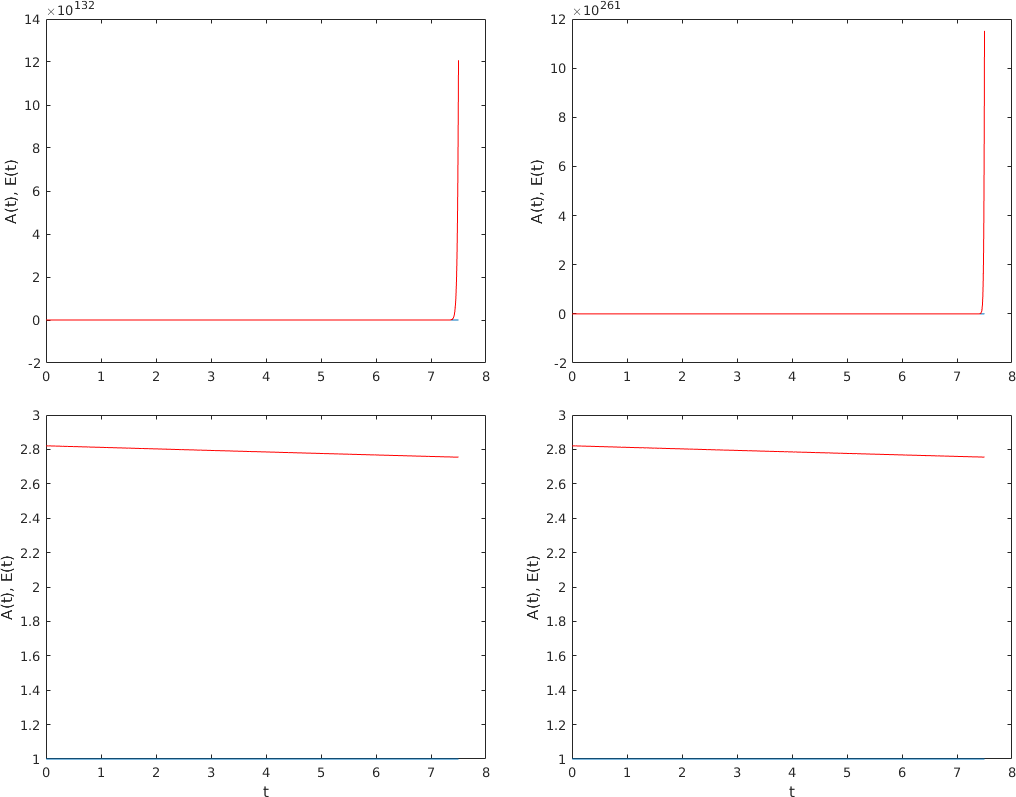
\includegraphics[scale=0.6]{./TEXT/conservation.png}
\caption{Illustration of the conservation for the default values}
\label{conservation}
\end{figure}